On this system, you find yourself caught up in the misadventures of
PlanEx, an
intergalactic delivery company led by the eccentric old mathematician
Dr. Farnswell. In the name of good relations between galaxies, you
agree to help him with the following puzzle. 

\begin{itemize}
\item PlanEx makes deliveries
to six different planets (not including their own) on Mondays, Wednesdays,
and Fridays. 
\item Each day, a different company on each planet receives the
delivery, listed below in order of Mon/Wed/Fri.
\begin{itemize}
\item Planet 1: Venus Co. / Rave Co. / Photon Co.
\item Planet 2: Comet Co. / Solar Co. / Light Co.
\item Planet 3: Belt Co. / Techno Co. / Alarm Co.
\item Planet 4: Acme Co. / Alpha Co. / Uranium Co.
\item Planet 5: Oxygen Co. / Helmet Co. / Neo Co.
\item Planet 6: Star Co. / Orion Co. / Tele Co.
\end{itemize}
\item Their ship may travel directly between any two planets,
  but due to galactic regulations, they may not travel directly
  between the same two planets twice in the same week, regardless
  of direction. This restriction includes travel to/from the Home Planet.
\end{itemize}

Can you help Farnswell complete his \textbf{Delivery Schedule}? If so,
the missing company names will reveal a hidden codeword. 

\begin{center}
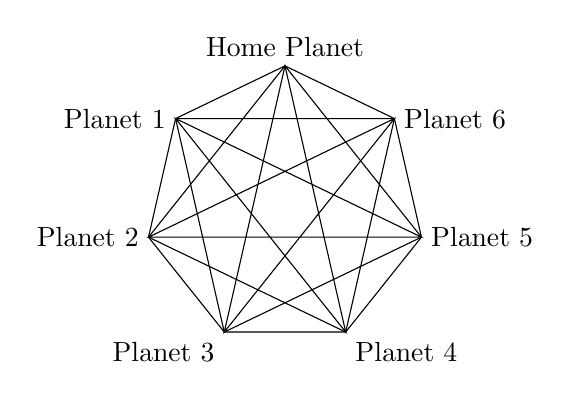
\begin{tikzpicture}[x=0.7in,y=0.7in]
\coordinate (Vertex0) at (90:1);
\coordinate (Vertex1) at (141.4:1);
\coordinate (Vertex2) at (192.9:1);
\coordinate (Vertex3) at (244.3:1);
\coordinate (Vertex4) at (295.7:1);
\coordinate (Vertex5) at (347.1:1);
\coordinate (Vertex6) at (38.6:1);
\node[above] at (Vertex0) {Home Planet};
\node[left] at (Vertex1) {Planet 1};
\node[left] at (Vertex2) {Planet 2};
\node[below left] at (Vertex3) {Planet 3};
\node[below right] at (Vertex4) {Planet 4};
\node[right] at (Vertex5) {Planet 5};
\node[right] at (Vertex6) {Planet 6};
\draw 
  (Vertex0) -- 
  (Vertex1) -- 
  (Vertex2) --
  (Vertex3) -- 
  (Vertex4) -- 
  (Vertex5) --
  (Vertex6) --
  cycle; 
\draw 
  (Vertex0) -- 
  (Vertex2) -- 
  (Vertex4) --
  (Vertex6) -- 
  (Vertex1) -- 
  (Vertex3) --
  (Vertex5) --
  cycle; 
\draw 
  (Vertex0) -- 
  (Vertex3) -- 
  (Vertex6) --
  (Vertex2) -- 
  (Vertex5) -- 
  (Vertex1) --
  (Vertex4) --
  cycle; 
\end{tikzpicture}
\end{center} 
